\documentclass{article}

\usepackage[hangul]{kotex}
\usepackage{amsmath}
\usepackage{tikz}
\usepackage{minted}
\usepackage{geometry}
\usepackage{enumitem}
\usepackage{multicol}
\usepackage[linguistics]{forest}
\usepackage{algorithm}
\usepackage{algpseudocode}
\usepackage{hyperref}

\hypersetup{
  colorlinks   = false, %Colours links instead of ugly boxes
  urlcolor     = blue, %Colour for external hyperlinks
  linkcolor    = black, %Colour of internal links
  citecolor   = red %Colour of citations
}

\geometry{
  a4paper,
  left=2.7cm,
  right=2.7cm,
  top=2.7cm,
  bottom=2.7cm,
}

\setmonohangulfont{D2Coding}

\title{프로그래밍과 문제해결 \\ Assignment \#3}
\author{무은재학부 박재원 (2024****)}
\date{\today}

\begin{document}

\begin{titlepage}
	\centering
	{\huge CSED101 프로그래밍과 문제해결\par}
	\vspace{0.5cm}
	{\LARGE Assignment \#3\par}
	\vspace{0.5cm}
	{\large \today\par}
	\vfill
  
  \begin{multicols}{2}
    \vphantom{}
    \columnbreak
  {
    \Large 
    \begin{description}[nosep, align=right, labelwidth=\widthof{00000000000000000}]
      \item[학과] 무은재학부
      \item[학번] 2024****
      \item[이름] 박재원
      \item[POVIS ID] ****
    \end{description}
  }
  \end{multicols}

  \vspace{1cm}


  \begin{quote}
    명예서약 (Honor code)

    ``나는 이 프로그래밍 과제를 다른 사람의 부적절한 도움 없이 완수하였습니다.''
  \end{quote}

\end{titlepage}

\tableofcontents

\section{개요}

본 과제는 슬롯머신 게임을 구현하는 것이다. 
Single Line Slot Game, Single Line with Wild Slot Game 두 가지 게임 규칙에 맞추어 
베팅, 스핀 및 보상 지급, 플레이어 정보 출력, 재화 재충전 등의 기능을 구현해야 한다.

\section{설계}

\subsection{구조도}

프로그램의 전체 구조도는 그림 \ref{fig:structurechart}와 같다. 

\begin{description}
  \item[입력부] 메뉴 선택 입력 받기(SelectUI.run)
  \item[처리부] 슬롯 게임 베팅 금액 관리 및 슬롯 진행, 재충전 기능, 종료 가능 여부 판단 등
  \item[출력부] 메뉴 출력, 슬롯 결과 출력, 현재 플레이어 정보 출력 등
\end{description}

\begin{figure}
  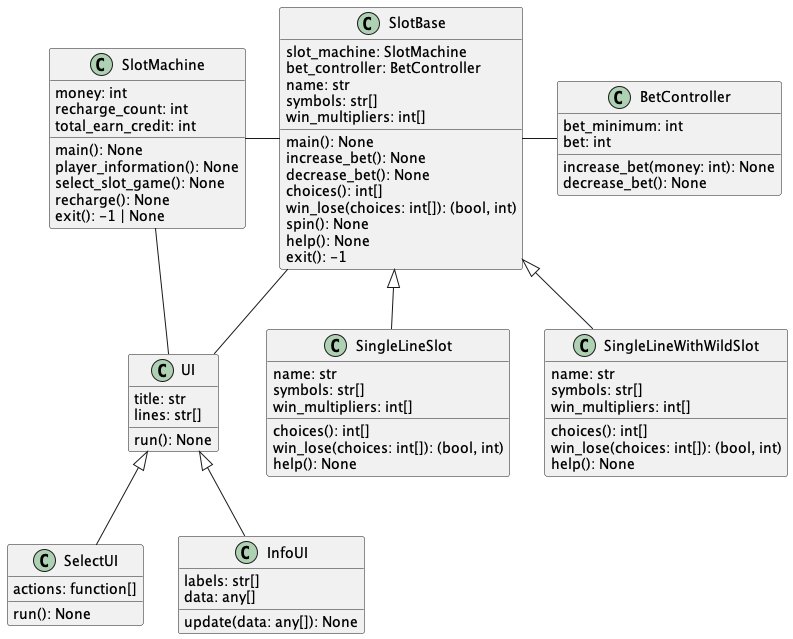
\includegraphics[width=\textwidth]{assets/structure_chart.png}
  \caption{본 프로그램의 전체 구조도}
  \label{fig:structurechart}
\end{figure}

\subsection{알고리즘}
프로그램의 알고리즘을 의사코드로 나타내면 알고리즘 \ref{alg:all}\과 같다.

\begin{algorithm}
  \caption{본 프로그램 주요 부분의 의사 코드} \label{alg:all}
  \begin{algorithmic}
    \While {}
      \State 메뉴 출력
      \State 입력값 $\gets$ 사용자 선택 입력 받기
      \If {입력값 $=$ 0}
        \State 현재 정보 출력
      \ElsIf {입력값 $=$ 1}
        \State 슬롯 게임 선택 및 실행
        \Comment 알고리즘 \ref{alg:slotgame} 참고
      \ElsIf {입력값 $=$ 2}
        \If {현재 돈 $<$ 500}
          \State 현재 돈 $\gets$ 1000
        \EndIf
      \ElsIf {입력값 $=$ 3}
        \If {총 획득한 돈 $> 5000$}
          \State 점수 출력 및 프로그램 종료(while문 break)
        \EndIf
      \EndIf
    \EndWhile
  \end{algorithmic}
\end{algorithm}

\begin{algorithm}
  \caption{슬롯 게임 의사 코드} \label{alg:slotgame}
  \begin{algorithmic}
    \State BetController 인스턴스 생성
    \While {}
      \State 메뉴 출력
      \State 입력값 $\gets$ 사용자 선택 입력 받기
      \If {입력값 $=$ 0}
        \State 스핀 시작 문구 출력
        \State 0.5초 대기
        \State 심볼 중에서 3개 뽑기 및 출력
        \State 0.2초 대기
        \If {승리 규칙에 부합}
          \State 승리 문구 및 획득한 돈 출력
        \Else
          \State 패배 문구 출력
        \EndIf
      \ElsIf {입력값 $=$ 1}
        \State BetController의 베팅 금액 2배
      \ElsIf {입력값 $=$ 2}
        \State BetController의 베팅 금액 $\frac{1}{2}$배
      \ElsIf {입력값 $=$ 3}
        \State 도움말 출력
      \ElsIf {입력값 $=$ 4}
        \State while문 break
      \EndIf
    \EndWhile
  \end{algorithmic}
\end{algorithm}

\section{실행 방법 및 예제}

본 과제는 MacOS\footnote{특정 OS에 종속적인 기능을 사용하지 않으므로 다른 운영체제에서도 정상 작동하리라 예상된다.}, CPython 3.12.2에서 작성 및 테스트되었다.

본 과제를 실행하려면 다음과 같이 assn3.py 파이썬 파일을 실행하면 된다.
프로그램이 실행되고 출력되는 메뉴에 따라 적절한 입력을 함으로써 프로그램을 사용할 수 있다.
\begin{minted}[]{bash}
  ls
  # assn3.py
  python assn3.py
  # ================================
  #  SlotMachine Game
  # ================================
  #  0. Player Information
  #  1. Select Slot Game
  #  2. Recharge
  #  3. Exit
  # ================================
  # Select:
\end{minted}

실제 프로그램 실행 모습은 그림 \ref{img:1} $\sim$ \ref{img:6}와 같다.

\begin{figure}
  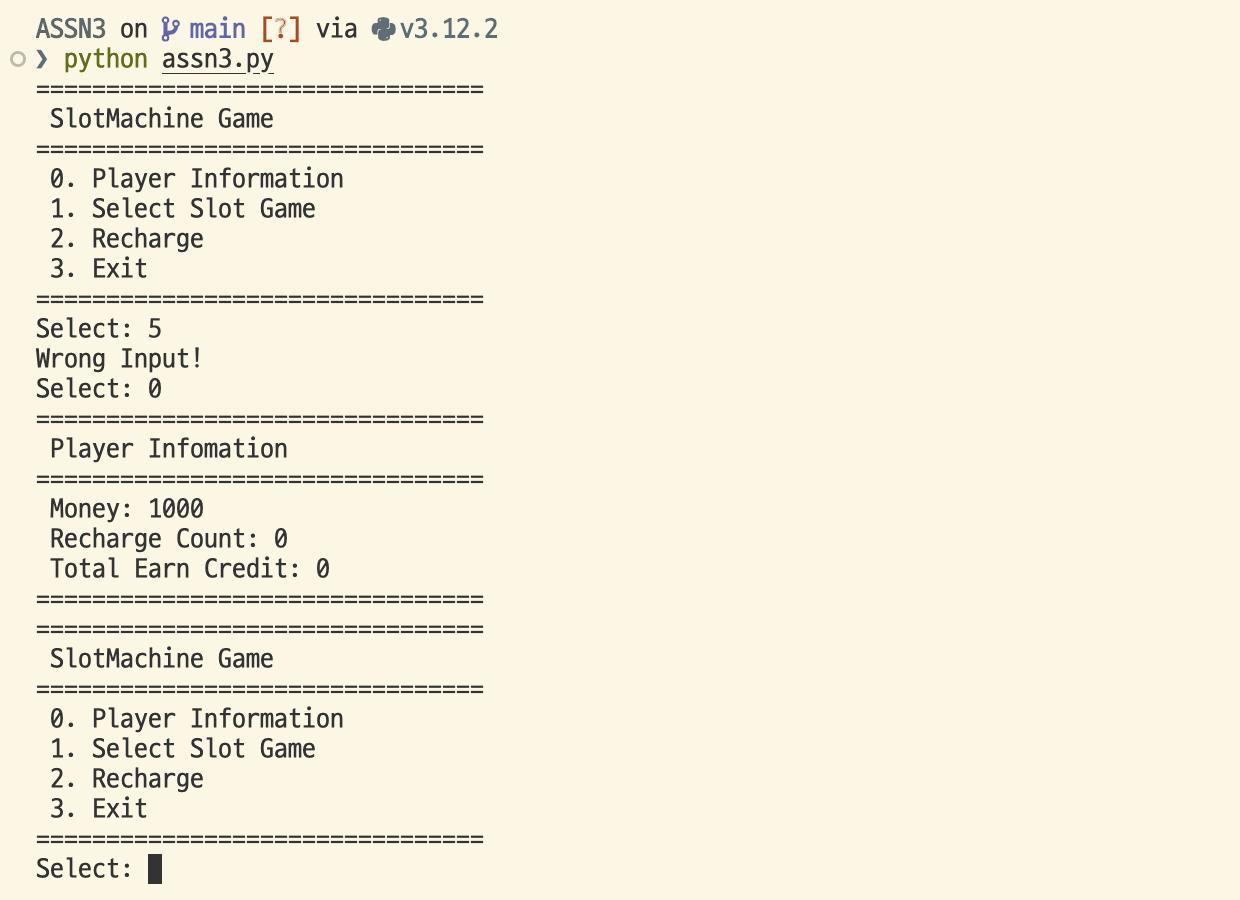
\includegraphics[width=\textwidth]{assets/screenshots/1.png}
  \caption{실행 모습. 초기 화면 및 플레이어 정보}
  \label{img:1}
\end{figure}
\begin{figure}
  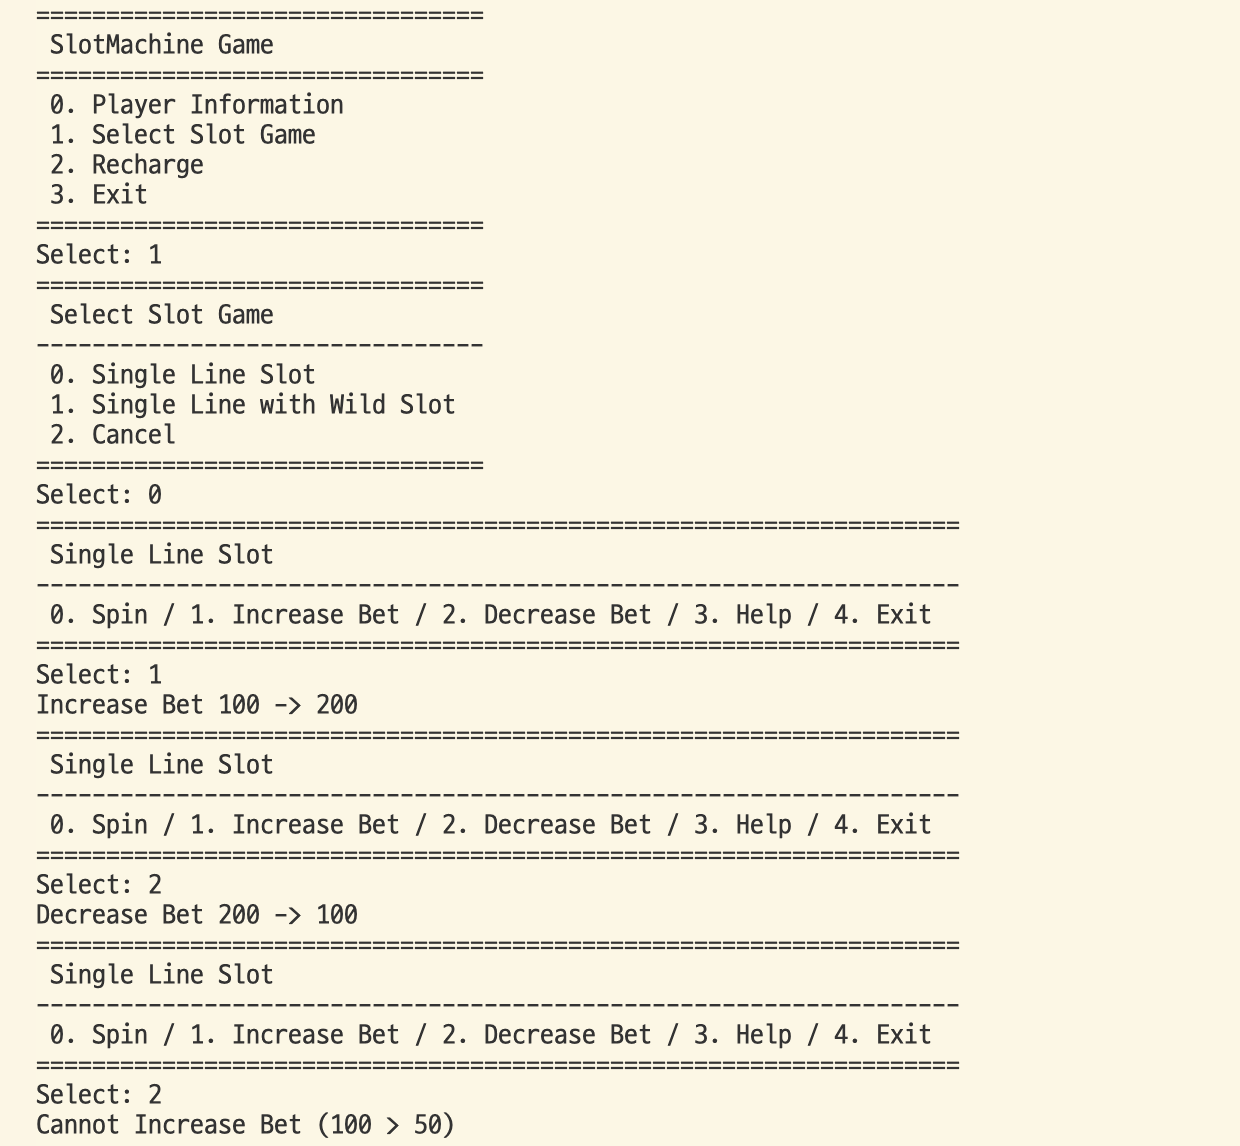
\includegraphics[width=\textwidth]{assets/screenshots/2.png}
  \caption{실행 모습. 슬롯 게임 선택 및 베팅 금액 조정}
  \label{img:2}
\end{figure}
\begin{figure}
  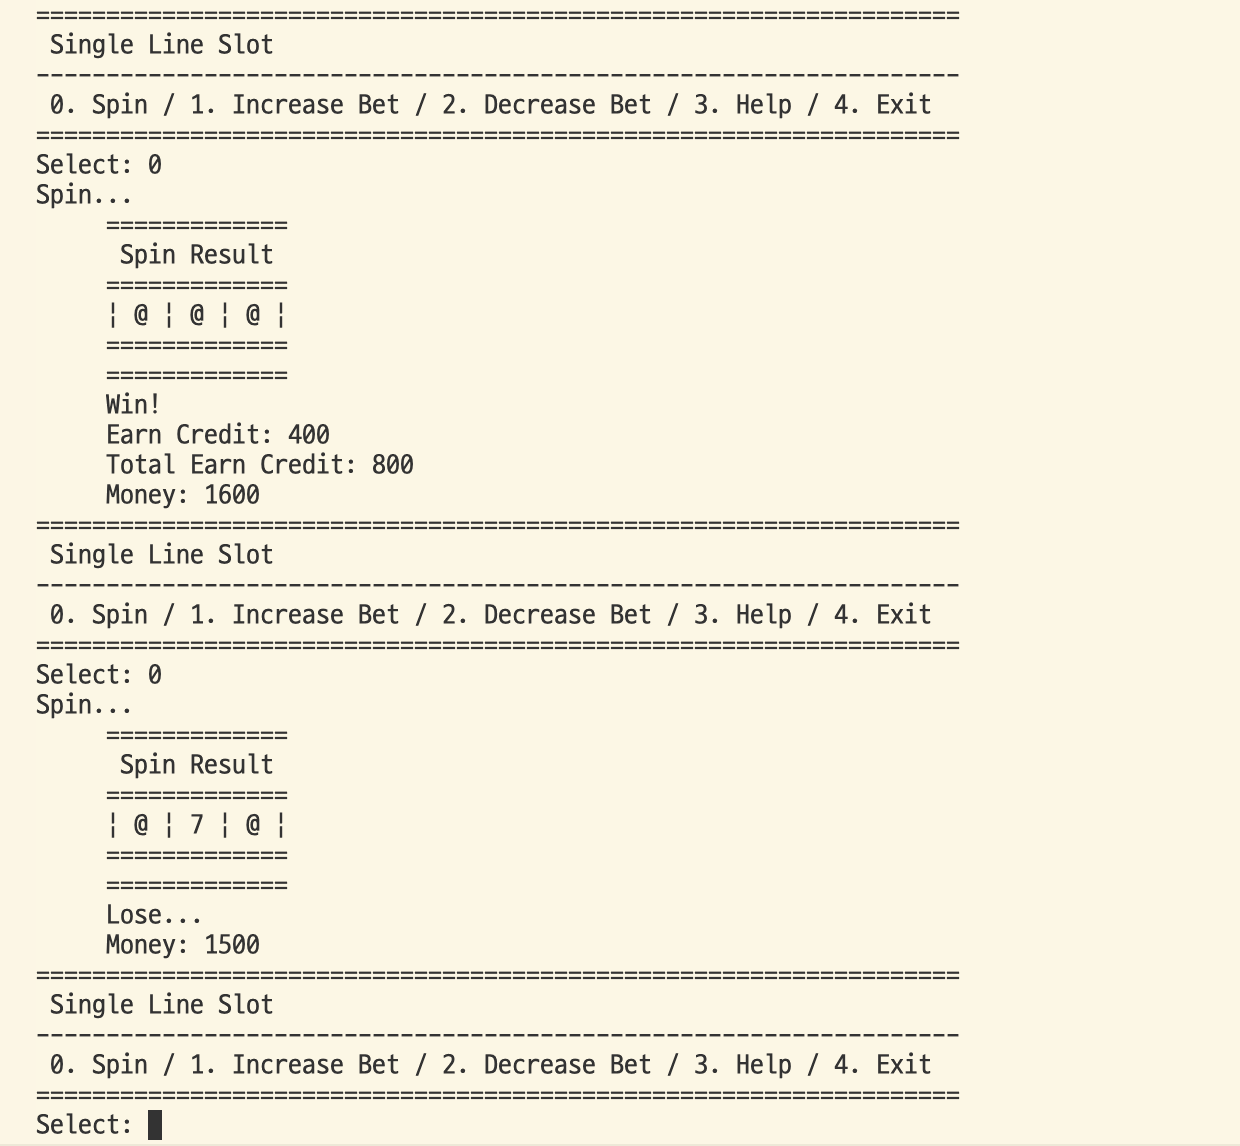
\includegraphics[width=\textwidth]{assets/screenshots/3.png}
  \caption{실행 모습. 스핀}
  \label{img:3}
\end{figure}
\begin{figure}
  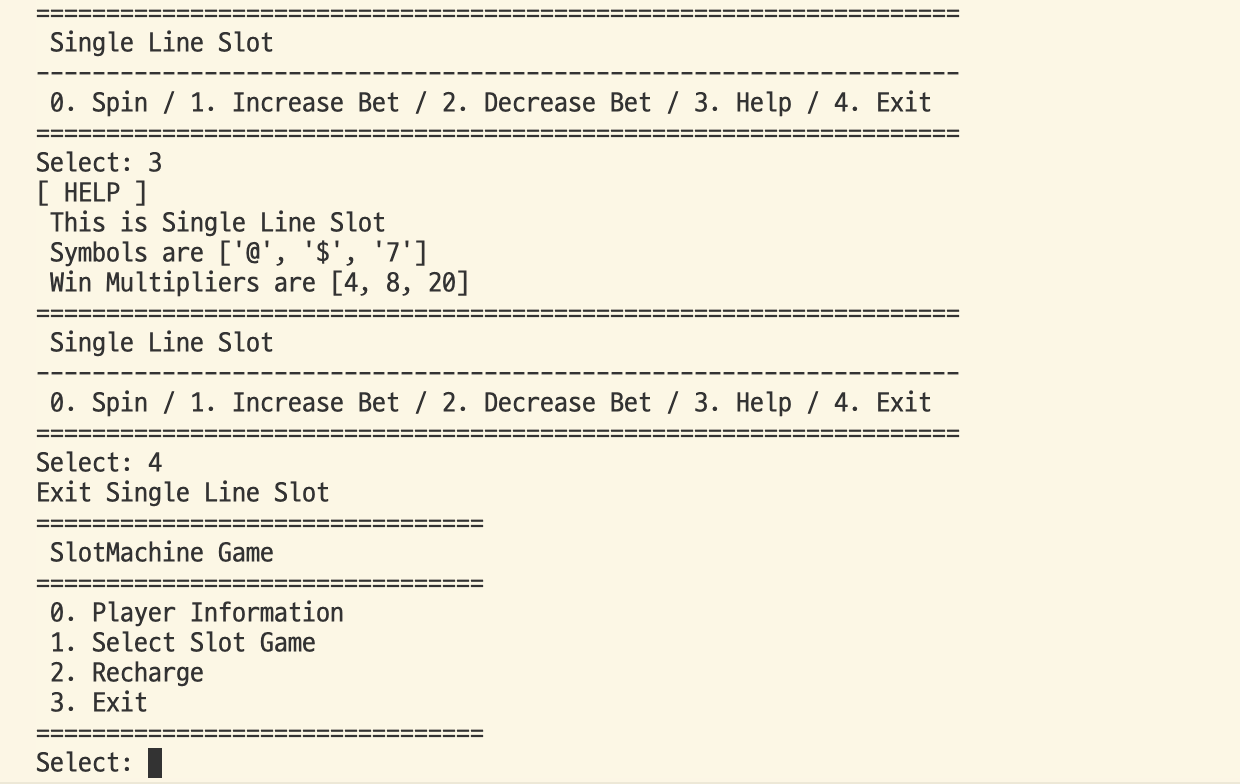
\includegraphics[width=\textwidth]{assets/screenshots/4.png}
  \caption{실행 모습. 슬롯 게임의 help, exit 실행 결과}
  \label{img:4}
\end{figure}
\begin{figure}
  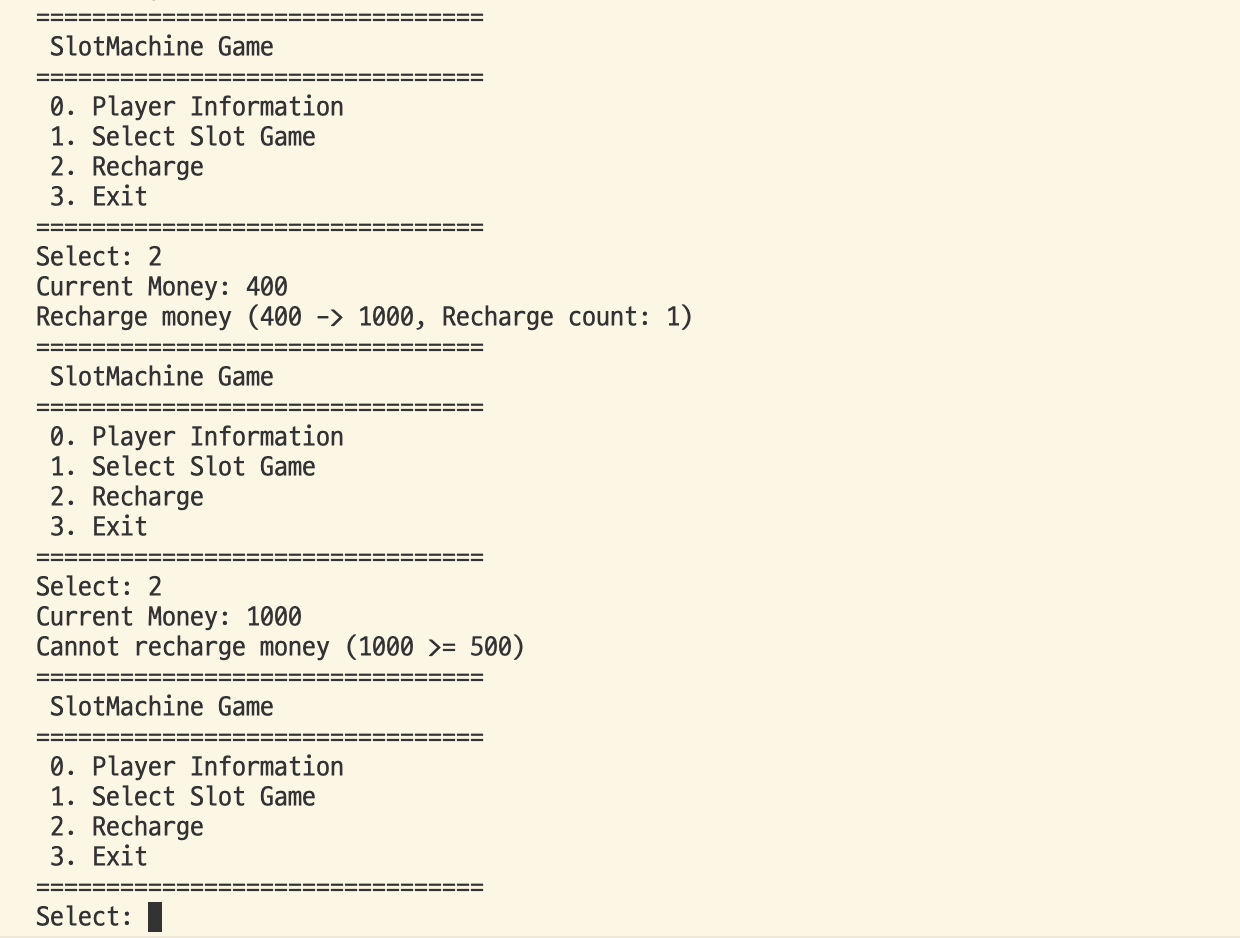
\includegraphics[width=\textwidth]{assets/screenshots/5.png}
  \caption{실행 모습. recharge 실행 결과}
  \label{img:5}
\end{figure}
\begin{figure}
  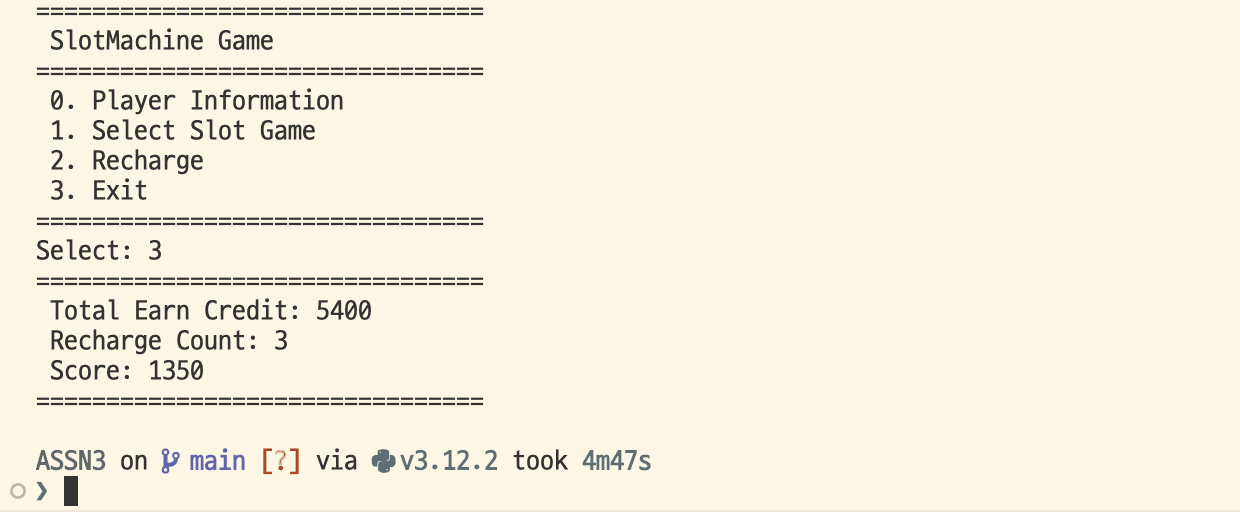
\includegraphics[width=\textwidth]{assets/screenshots/6.png}
  \caption{실행 모습. exit 실행 결과}
  \label{img:6}
\end{figure}

\begin{itemize}
  \item 그림 \ref{img:1}\은 실행 직후 기본 메뉴 출력 모습, 잘못된 입력 시 에러 처리, 0번 선택 시 플레이어 정보 출력 파트를 보여주고 있다.
  \item 그림 \ref{img:2}\은 기본 메뉴에서 1번을 선택해 슬롯 선택으로 이동해 Single Line Slot을 선택한 모습, 베팅 금액을 조절하는 모습이다. 배팅 금액은 100 이하로 내려가지 않음을 볼 수 있다.
  \item 그림 \ref{img:3}\은 Single Line Slot 스핀 돌리는 모습이다. 처음에는 승리해서 베팅금액($100$) $\times$ 보상 배수 ($4$) $= 400$을 획득했음을 알 수 있다. 두번 째에는 패배해서 베팅 금액($100$)을 잃었음을 알 수 있다.
  \item 그림 \ref{img:4}\은 3번을 선택해 도움말을 출력한 모습과, 4번을 선택해 exit한 모습이다. exit 하면 초기 기본 메뉴로 돌아간다. 
  \item 그림 \ref{img:5}\은 기본 메뉴에서 2번을 선택해 재충전하는 모습이다. 처음에는 돈이 500 미만으로 남아서 재충전이 이루어졌고, 재충전 카운트가 증가했다. 2번 째 시도에서는 돈이 500 이상이여서 재충전되지 않았다. 
  \item 그림 \ref{img:6}\은 기본 메뉴에서 3번을 선택해 종료를 시도하는 모습이다. 총 획득 돈이 5000을 넘겨서 성공적으로 종료되었다. 종료 시 점수를 계산해 출력한다.
\end{itemize}

\section{토론}

\subsection{spin 구현}

문제 파일에는 spin 메소드를 child class에 구현하라고 명시되어 있지만,
심볼 선택, 승패 판단을 제외한 텍스트 출력, 대기 등의 로직은 동일하기 때문에
이를 반복해 작성하는 것은 비효율적이라고 판단했다.

따라서 SlotBase 클래스에 choices 메소드(심볼 선택)와 win\_lose 메소드(승패 판단)를 새롭게 추가하고, child class에서 이 메소드들을 오버라이딩함으로써 게임 마다 차이가 나는 로직을 구현했다.
공통된 로직은 SlotBase 클래스의 slot 메소드에 구현하고, 그 안에서 choices, win\_lose 메소드를 호출하도록
구현함으로써 각 게임 규칙에 맞는 동작을 하면서 동시에 코드 중복을 최소화하였다.

\subsection{UI 출력}

고정된 형식의 UI를 출력할 일이 많아 이를 별도 class로 정의해 사용했다.
기본적인 기능을 담은 UI 클래스, 이를 상속받은 SelectUI와 InfoUI 클래스를 만들었다.
SelectUI는 사용자로부터 선택을 입력받는 메뉴, InfoUI는 변수의 값을 출력하는 UI에 사용한다.
UI의 제목, 내용 리스트 등을 인자로 넘겨 인스턴스를 생성하고, run 메소드를 실행하면 UI가 출력된다.

\section{결론}

파이썬에서 클래스를 정의하고 사용해봄으로써 객체 지향 프로그래밍을 연습해보았다.
클래스 상속, 메소드 오버라이딩 등 여러 기법도 사용해 볼 수 있었다.
이를 통해 객체 지향 프로그래밍에 익숙해질 수 있었다.

\section{개선 방향}

슬롯 게임의 help 메뉴를 선택 시 심볼 등만 출력하는 것이 아니라,
승리 조건 등 자세한 내용을 더 출력하도록 개선하면 사용자에게 더 친절한 프로그램이 될 것이라 생각한다.

또한 더 다양한 규칙의 슬롯 게임을 추가하는 방향으로 개선하는 것도 좋겠다.

\end{document}